\documentclass[10pt,twocolumn,letterpaper]{article}

\usepackage[margin=0.75in,columnsep=0.25in]{geometry}
\usepackage{times}
\usepackage{amsmath,amssymb,amsfonts}
\usepackage{booktabs}
\usepackage{graphicx}
\usepackage{xcolor}
\usepackage{tikz}
\usepackage{pgfplots}
\usepackage{caption}
\usepackage{subcaption}
\usepackage{algorithm}
\usepackage{algpseudocode}
\usepackage{microtype}
\usepackage[colorlinks=true,linkcolor=black,citecolor=black,urlcolor=blue]{hyperref}

\pgfplotsset{compat=1.18}
\usetikzlibrary{arrows.meta,positioning,fit,backgrounds,calc,patterns}

% ---- palette -------------------------------------------------------------
\definecolor{ctx}{HTML}{2B6CB0}      % context / given
\definecolor{gen}{HTML}{C05621}      % generated / masked
\definecolor{frz}{HTML}{718096}      % frozen
\definecolor{trn}{HTML}{2F855A}      % trained
\definecolor{bg}{HTML}{EDF2F7}

\newcommand{\R}{\mathbb{R}}
\newcommand{\bx}{\mathbf{x}}
\newcommand{\bz}{\mathbf{z}}
\newcommand{\bm}{\mathbf{m}}
\newcommand{\bef}{\boldsymbol{\epsilon}}

\title{\vspace{-2em}\textbf{Outpainting Audio by Reusing What the Model Already Knows:\\
A Minimal Full-Finetune Recipe for Latent Rectified-Flow Audio Diffusion}}

\author{Francesco Colonnese\\
\texttt{github.com/mrcolo/loop-training}}

\date{}

\begin{document}
\maketitle

\begin{abstract}
Audio outpainting --- continuing a recording past its end --- is usually framed as a
new capability requiring new machinery: extra input channels, adapter branches, or a
separately trained continuation head. We observe that a modern latent audio diffusion
model already contains everything the task needs. Stable Audio 3 Medium is trained with
inpainting conditioning, taking a binary mask and a masked latent as local-additive
conditions, and its mask distribution already includes a \emph{causal} mode that retains
a random-length prefix. Outpainting is that mode. Consequently a finetune for
outpainting can change \emph{no architecture at all}: no new channels, no adapters, no
surgery on the input projection. Only the transformer weights move.

The recipe that follows is complete, targets a single 24\,GB consumer GPU, and trains
all 1.453\,B transformer parameters. Its central finding is about \emph{which} published
weights admit it. The model ships in two forms, a rectified-flow checkpoint and the
adversarially post-trained checkpoint used for eight-step inference, and a squared-error
finetune is valid only on the first. We show that the post-trained weights encode a
\emph{sample} predictor, that a thousand squared-error steps convert them into a
conditional-mean predictor, and that the eight-step sampler cannot tolerate the
difference. The conversion is invisible to every scalar in the training log --- loss
falls monotonically throughout --- and is measurable in one forward pass by comparing
the scale of the one-step estimate to its correlation with the truth. We give that
diagnostic, the corrected recipe, and the memory budget that makes it fit.
\end{abstract}

% ==========================================================================
\section{Introduction}

Generative audio models have converged on latent diffusion: a high-compression
autoencoder maps waveforms to a short sequence of continuous vectors, and a diffusion
transformer (DiT) is trained in that space. The recipe is now mature enough that the
interesting questions have shifted from \emph{how to generate} to \emph{how to control},
and one of the most practically useful controls is continuation: given the first
$\tau$ seconds of a recording, produce what plausibly follows.

The standard reflex is to treat this as an architectural problem. Image inpainting
models concatenate a mask and a masked image to the noisy latent, widening the input
projection from $C$ to $2C{+}1$ channels and zero-initialising the new columns. The same
construction transfers to audio and works. But it is unnecessary when the base model was
already trained with masked conditioning.

\begin{figure}[t]
\centering
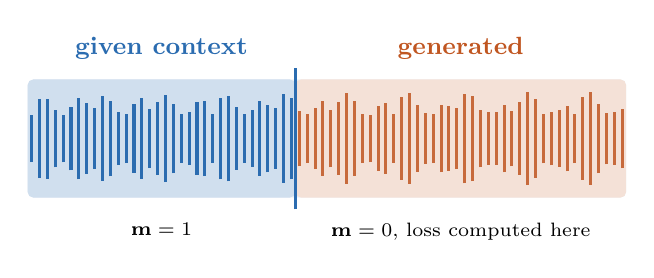
\begin{tikzpicture}[scale=1.0]
% waveform-ish context
\fill[bg,rounded corners=2pt] (0,0) rectangle (7.6,1.5);
\fill[ctx!22,rounded corners=2pt] (0,0) rectangle (3.4,1.5);
\fill[gen!18,rounded corners=2pt] (3.4,0) rectangle (7.6,1.5);
\draw[ctx,thick] (3.4,-0.15) -- (3.4,1.65);

% pseudo waveform: context solid, generation dashed
\foreach \i in {0,...,33}{
  \pgfmathsetmacro{\h}{0.30+0.30*abs(sin(\i*47))*abs(cos(\i*23))}
  \draw[ctx,line width=1.1pt] ({0.05+\i*0.1},{0.75-\h}) -- ({0.05+\i*0.1},{0.75+\h});
}
\foreach \i in {34,...,75}{
  \pgfmathsetmacro{\h}{0.30+0.30*abs(sin(\i*47))*abs(cos(\i*23))}
  \draw[gen,line width=1.1pt,opacity=0.85] ({0.05+\i*0.1},{0.75-\h}) -- ({0.05+\i*0.1},{0.75+\h});
}
\node[ctx,font=\small\bfseries] at (1.7,1.9) {given context};
\node[gen,font=\small\bfseries] at (5.5,1.9) {generated};
\node[font=\scriptsize,anchor=north] at (1.7,-0.2) {$\bm=1$};
\node[font=\scriptsize,anchor=north] at (5.5,-0.2) {$\bm=0$, loss computed here};
\end{tikzpicture}
\caption{\textbf{The task.} A random-length prefix of a latent sequence is retained as
context; the model generates the remainder. This is exactly the \emph{causal} member of
the mask family the base model was pretrained with, so no architectural change is
required. The training loss is taken only over the generated region.}
\label{fig:teaser}
\end{figure}

\paragraph{Contributions.} (i) We identify that outpainting is a \emph{subset} of the
inpainting conditioning already present in Stable Audio 3, and show that restricting the
pretrained mask distribution toward its causal mode is sufficient to specialise the model
for continuation (\S\ref{sec:mask}). (ii) We show that squared-error training on an
adversarially post-trained checkpoint silently converts a sample predictor into a
conditional-mean predictor, give a one-forward-pass diagnostic that detects it, and
report the failure it produces in full (\S\ref{sec:checkpoint}).
(iii) We argue that the optimiser is part of the recipe rather than an implementation
detail, and that an orthogonalised update is what makes a single learning rate valid
across a transformer's matrices (\S\ref{sec:opt}). (iv) We give a memory budget under
which all 1.453\,B transformer parameters, an orthogonalising optimiser and a weight
average fit on one 24\,GB GPU (\S\ref{sec:memory}), and a data path with no manifest and
no preprocessing stage (\S\ref{sec:data}). (v) We argue that per-step training loss is
the wrong instrument for this objective and propose a frozen evaluation slice
(\S\ref{sec:eval}) --- while showing that even a well-behaved validation curve is not
sufficient.

% ==========================================================================
\section{Related Work}

\paragraph{Latent audio diffusion.} Encoding waveforms into a compact latent sequence
before diffusion is now standard, and the compression ratio has risen sharply: the
autoencoder we build on maps $4096$ waveform samples to a single $256$-dimensional latent
frame, a $10.77$\,Hz representation of $44.1$\,kHz stereo. High compression is what makes
minute-scale generation tractable, and it is also what makes online encoding expensive
(\S\ref{sec:cost}).

\paragraph{Masked generative modelling.} Inpainting by channel-concatenating a mask and a
masked signal originates in image diffusion and has been carried into audio. The variant
we exploit differs in that the masked conditioning is injected as a \emph{local additive}
term rather than by widening the input projection, and --- critically --- is present at
pretraining rather than bolted on afterwards.

\paragraph{Flow matching and rectified flow.} Rectified flow replaces the variance-
preserving diffusion path with a straight interpolation between data and noise, and
predicts the constant velocity along it. Its simplicity and its compatibility with
few-step distilled samplers have made it the default for recent audio models.

\paragraph{Full versus parameter-efficient finetuning.} LoRA and adapters dominate
finetuning practice because they fit on small hardware. We take the opposite position for
this task: when the target domain differs from the pretraining distribution in timbre and
production style rather than in semantics, the low-rank constraint is a real limitation,
and a 1.45\,B model \emph{can} be fully finetuned on a consumer card given the right
precision and optimiser-state choices.

% ==========================================================================
\section{Preliminaries}

\subsection{Latent representation}

Let $\bx \in \R^{2 \times N}$ be stereo audio at $44.1$\,kHz. A frozen autoencoder
$\mathcal{E}$ maps it to
\begin{equation}
\bz = \mathcal{E}(\bx) \in \R^{256 \times T}, \qquad T = \lceil N / 4096 \rceil ,
\end{equation}
a $256$-channel sequence at $10.77$ frames per second. The encoder is a patched
transformer: waveform samples are first grouped into patches of $256$, then a
$12$-layer transformer with stride $16$ produces the latent. The decoder mirrors it.
Together they account for $0.852$\,B parameters and remain frozen throughout.

\subsection{Rectified-flow objective}

The generative model is a DiT $v_\theta$ trained with a rectified-flow ($\texttt{rf\_denoiser}$)
objective. For $t \in [0,1]$ and $\bef \sim \mathcal{N}(0, I)$,
\begin{align}
\bz_t &= (1-t)\,\bz + t\,\bef, \label{eq:path}\\
v^\star &= \bef - \bz, \label{eq:target}
\end{align}
so that $t{=}0$ is data and $t{=}1$ is noise, and the target velocity is constant along
each path. The network is conditioned on $t$, on a text embedding, and on a scalar
duration embedding.

\begin{figure}[t]
\centering
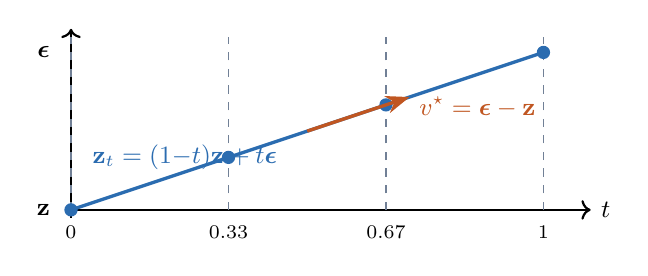
\begin{tikzpicture}[scale=1.0]
\draw[->,thick] (0,0) -- (6.6,0) node[right,font=\small] {$t$};
\draw[->,thick] (0,-0.1) -- (0,2.3);
\node[font=\small] at (-0.35,0) {$\bz$};
\node[font=\small] at (-0.35,2.0) {$\bef$};
% straight interpolation
\draw[ctx,very thick] (0,0) -- (6.0,2.0);
\foreach \x/\l in {0/0, 2/0.33, 4/0.67, 6/1}{
  \draw[frz,dashed] (\x,0) -- (\x,2.2);
  \node[font=\scriptsize,anchor=north] at (\x,-0.08) {\l};
}
\foreach \x in {0,2,4,6}{
  \pgfmathsetmacro{\y}{\x/3.0}
  \fill[ctx] (\x,\y) circle (2.4pt);
}
% velocity arrow
\draw[gen,-{Stealth[length=3mm]},very thick] (3.0,1.0) -- ++(1.3,0.433);
\node[gen,font=\small,anchor=west] at (4.3,1.30) {$v^\star=\bef-\bz$};
\node[ctx,font=\small,anchor=north west] at (0.15,0.95) {$\bz_t=(1{-}t)\bz+t\bef$};
\end{tikzpicture}
\caption{\textbf{Rectified flow.} Data and noise are joined by a straight line, and the
network regresses the constant velocity along it. Because the path is linear, the
velocity target does not depend on $t$ --- but the \emph{difficulty} of predicting it
does, which is the source of the variance discussed in \S\ref{sec:eval}.}
\label{fig:rf}
\end{figure}

\subsection{Timestep sampling}

Timesteps are drawn from a truncated logistic-normal distribution, reflected, and then
warped by a sequence-length-dependent shift $\sigma_L$ that moves probability mass toward
higher noise for longer sequences:
\begin{equation}
t \sim \sigma_L\big(1 - \mathrm{TLN}(0.075, 1)\big).
\end{equation}
We reuse the pretraining sampler unchanged. Matching it matters: a finetune that samples
timesteps differently from pretraining spends its gradient budget on a different part of
the schedule than the one the model was optimised for.

\begin{figure}[t]
\centering
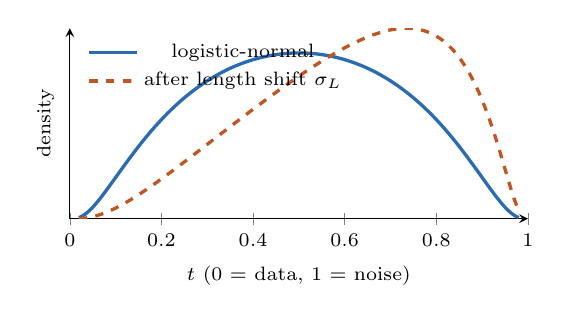
\begin{tikzpicture}
\begin{axis}[
  width=7.4cm, height=4.0cm,
  xlabel={$t$ (0 = data, 1 = noise)},
  ylabel={density},
  xmin=0, xmax=1, ymin=0,
  ytick=\empty,
  tick label style={font=\scriptsize},
  label style={font=\scriptsize},
  legend style={font=\scriptsize,draw=none,fill=none,at={(0.02,0.98)},anchor=north west},
  axis lines=left,
]
\addplot[ctx,very thick,domain=0.02:0.98,samples=120,smooth]
  {exp(-0.5*(ln(x/(1-x)))^2)/(x*(1-x))*0.4};
\addlegendentry{logistic-normal}
\addplot[gen,very thick,dashed,domain=0.02:0.98,samples=120,smooth]
  {exp(-0.5*(ln(x/(1-x))-0.55)^2)/(x*(1-x))*0.4};
\addlegendentry{after length shift $\sigma_L$}
\end{axis}
\end{tikzpicture}
\caption{\textbf{Timestep density.} Mass concentrates in the middle of the schedule where
the prediction problem is hardest, and the length-dependent shift moves it toward higher
noise as the sequence grows. We inherit both from pretraining rather than substituting a
uniform sampler.}
\label{fig:tdist}
\end{figure}

% ==========================================================================
% ==========================================================================
\section{Which checkpoint admits a squared-error finetune}
\label{sec:checkpoint}

Stability publishes two weights for this model, and the choice between them is
the single decision that determines whether the finetune works at all.

\textsc{Base} is the rectified-flow model: it predicts a velocity, and it is
sampled with an ODE solver in roughly $50$ steps with classifier-free guidance.
\textsc{Released} is that model after adversarial post-training. It predicts a
\emph{sample} rather than a conditional mean, and it is sampled with ping-pong in
$8$ steps at guidance $1$:
\begin{align}
\hat\bz_0 &= \bz_t - t\, v_\theta(\bz_t, t, c), \label{eq:pp1}\\
\bz_{t'}  &= (1-t')\,\hat\bz_0 + t'\,\bm{\epsilon}',\quad \bm{\epsilon}'\sim\mathcal{N}(0,I).
\label{eq:pp2}
\end{align}
Equation~\eqref{eq:pp2} discards the previous iterate entirely and rebuilds it
from $\hat\bz_0$ and fresh noise. Every step therefore requires $\hat\bz_0$ to be
a full-scale, self-consistent clip \emph{on its own}, at every noise level.

A squared-error objective does not produce that. Its minimiser is
$\mathbb{E}[\bz_0 \mid \bz_t]$, whose scale shrinks exactly in proportion to how
much the model actually knows: if $\rho$ is the correlation between the estimate
and the truth, then $\operatorname{std}(\hat\bz_0)/\operatorname{std}(\bz_0)
\rightarrow \rho$. A sample predictor instead holds that ratio near $1$ even
where $\rho$ is small. The two are distinguishable in a single forward pass.

\begin{table}[t]
\centering
\small
\begin{tabular}{lcccc}
\toprule
& \multicolumn{2}{c}{\textsc{Released}} & \multicolumn{2}{c}{$+\,1000$ MSE steps} \\
\cmidrule(lr){2-3}\cmidrule(lr){4-5}
$t$ & std ratio & $\rho$ & std ratio & $\rho$ \\
\midrule
$0.95$ & \textbf{0.832} & 0.321 & \textbf{0.551} & 0.502 \\
$0.90$ & 0.896 & 0.565 & 0.686 & 0.662 \\
$0.80$ & 0.964 & 0.719 & 0.784 & 0.785 \\
$0.60$ & 0.999 & 0.872 & 0.892 & 0.899 \\
$0.40$ & 1.004 & 0.946 & 0.948 & 0.954 \\
$0.20$ & 1.001 & 0.985 & 0.983 & 0.986 \\
\bottomrule
\end{tabular}
\caption{Scale of the one-step estimate $\hat\bz_0$ relative to the truth, against
its correlation with the truth, on a real excerpt under a full mask. The released
checkpoint emits a full-scale sample where it knows almost nothing. After a
thousand squared-error steps the two columns coincide at every noise level, which
is the defining signature of a conditional-mean predictor.}
\label{tab:probe}
\end{table}

Table~\ref{tab:probe} runs that test. A thousand squared-error steps convert the
released checkpoint into a mean predictor: the two columns become equal
throughout. At the first ping-pong step the generated signal has lost a third of
its amplitude while \eqref{eq:pp2} continues to inject noise at full scale.
Perceptually the output flattens and hisses.

Two things make this failure difficult to catch. First, the correlation
\emph{improves}, $0.321 \rightarrow 0.502$ at $t=0.95$: the model is getting
better at the objective it was given, and validation loss falls monotonically
throughout. Second, no scalar in the training log distinguishes the two regimes;
the diagnostic has to be constructed deliberately.

The mechanism is not incidental --- it is the stated purpose of the post-training
stage, which works ``by supplanting the MSE-based conditional mean loss \dots\
with an adversarial loss''. Running squared error on those weights re-imposes the
loss the stage was run to remove, and no learning rate makes that objective
correct; a smaller one only slows the regression. Stability's own trainer refuses
the released checkpoint outright, and their documentation gives the remedy:
adapters ``are trained on the base checkpoint. Once trained, they can be applied
to the post-trained model and will work as expected.'' We therefore train
\textsc{Base}, store checkpoints as the \emph{delta} from its weights, and add
that delta to \textsc{Released} at inference. The same rule is established in
images: a distilled model is ``impossible to train on directly because every step
you train breaks down the compression more and more''.


\subsection{The delta transplants}
\label{sec:transplant}

Training \textsc{Base} is only useful if the result can be moved onto
\textsc{Released}, and the guidance that says it can is written for low-rank
adapters, which are small by construction. A full finetune is not. Fetching one
transformer layer of \textsc{Released} by byte range and comparing it with
\textsc{Base} puts a number on the margin: adversarial post-training moved that
layer's weights by $1.38\%$ on median, and after 1000 steps our update is already
$0.85\times$ that, with two tensors past it. The question is therefore empirical.

Table~\ref{tab:transplant} answers it with the same diagnostic, run on four
models under identical noise. \textsc{Base} sits exactly on the conditional-mean
line, $0.535$ against $0.533$, and stays there once our delta is added, which is
correct: that is the objective it was trained with. \textsc{Released} separates
sharply, and \emph{keeps separating after the delta is added}: $0.965$ against
$0.408$, against $0.920$ and $0.393$ for the untouched weights. The few-step
behaviour is intact. Its correlation with the truth also rises, so the finetune's
knowledge of the target domain transfers into the accelerated model rather than
merely surviving in it.

\begin{table}[t]
\centering
\small
\begin{tabular}{lcccc}
\toprule
& $t{=}0.95$ & $t{=}0.9$ & $t{=}0.8$ & $t{=}0.6$ \\
\midrule
\textsc{Base}              & 0.535/0.533 & 0.605/0.605 & 0.735/0.740 & 0.869/0.873 \\
\textsc{Base} $+\,\Delta$  & 0.578/0.558 & 0.639/0.626 & 0.757/0.753 & 0.879/0.877 \\
\textsc{Released}          & 0.920/0.393 & 0.937/0.483 & 0.971/0.658 & 0.999/0.842 \\
\textbf{\textsc{Released} $+\,\Delta$} & \textbf{0.965/0.408} & 0.952/0.506 & 0.967/0.681 & 0.995/0.849 \\
\bottomrule
\end{tabular}
\caption{Amplitude / correlation of the one-step estimate, at 3000 finetuning
steps. Equal entries denote a conditional-mean predictor. The transplanted model
retains the separation that few-step sampling depends on.}
\label{tab:transplant}
\end{table}

The practical consequence is that the two checkpoints divide labour cleanly:
\textsc{Base} is what the objective is valid against, \textsc{Released} is what
inference runs on, and the finetune is transported between them as a float16
delta. Nothing about the recipe needs to change to get both.

% ==========================================================================
\section{Method}

\subsection{Outpainting as a restriction of pretrained masking}
\label{sec:mask}

The base model consumes two extra conditioning tensors alongside the noisy latent: a
binary keep-mask $\bm \in \{0,1\}^{1 \times T}$ and the masked latent $\bz \odot \bm$.
These enter the transformer as a local additive term of dimension $256{+}1$, added to the
token embeddings rather than concatenated to the input channels.

During pretraining, $\bm$ is drawn from a family of mask types. Three matter here:

\begin{description}\itemsep2pt
\item[\textsc{Full}] $\bm = 0$ everywhere. Pure unconditional generation.
\item[\textsc{Spans}] a set of non-overlapping interior spans is zeroed. General inpainting.
\item[\textsc{Causal}] a prefix length $k \sim \mathcal{U}\{0,\dots,T\}$ is sampled and
$\bm_{i} = \mathbf{1}[i < k]$. \textbf{This is outpainting.}
\end{description}

\begin{figure}[t]
\centering
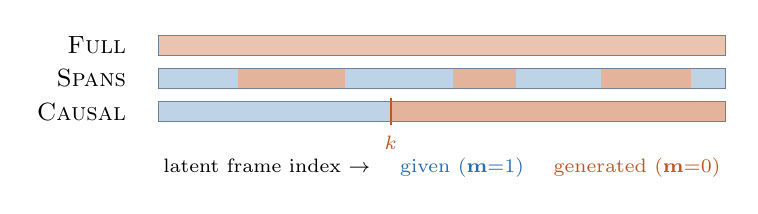
\begin{tikzpicture}[x=0.072cm,y=0.42cm]
\foreach \row/\name/\yy in {0/\textsc{Full}/0, 1/\textsc{Spans}/-1, 2/\textsc{Causal}/-2}{
  \node[anchor=east,font=\small] at (-4,\yy) {\name};
}
% FULL
\fill[gen!35] (0,-0.3) rectangle (100,0.3);
% SPANS
\fill[ctx!30] (0,-1.3) rectangle (100,-0.7);
\fill[gen!45] (14,-1.3) rectangle (33,-0.7);
\fill[gen!45] (52,-1.3) rectangle (63,-0.7);
\fill[gen!45] (78,-1.3) rectangle (94,-0.7);
% CAUSAL
\fill[ctx!30] (0,-2.3) rectangle (100,-1.7);
\fill[gen!45] (41,-2.3) rectangle (100,-1.7);
\draw[gen,thick] (41,-2.42) -- (41,-1.58);
\node[font=\scriptsize,anchor=north,gen] at (41,-2.45) {$k$};
\foreach \y in {0,-1,-2}{ \draw[frz,thin] (0,\y-0.3) rectangle (100,\y+0.3); }
\node[font=\scriptsize,anchor=north] at (50,-3.1)
  {latent frame index $\rightarrow$ \quad
   \textcolor{ctx}{given ($\bm{=}1$)} \quad \textcolor{gen}{generated ($\bm{=}0$)}};
\end{tikzpicture}
\caption{\textbf{The pretrained mask family.} Stable Audio 3 is pretrained with mask-type
probabilities $[0.1, 0.8, 0.1]$ over $[\textsc{Spans},\textsc{Full},\textsc{Causal}]$.
Outpainting is already in the support of this distribution --- it is simply rare. Our
finetune reweights to $[0, 0.1, 0.9]$.}
\label{fig:masks}
\end{figure}

Because \textsc{Causal} is already in the support of the pretraining distribution, the
finetune is a \emph{reweighting} rather than an extension. We set the mask-type
probabilities to $[0, 0.1, 0.9]$, concentrating gradient on continuation while retaining
a tenth of each batch at \textsc{Full}. That residual matters: training exclusively on
causal masks steadily degrades the model's unconditional behaviour, which is also the
behaviour the $\textsc{Full}$ branch of classifier-free guidance relies on at sampling
time.

\subsection{Two-term objective}

The report is explicit that the loss is not taken on the generated region alone:
it ``is split into two independently averaged terms: a generation loss over the
inpainted embeddings ($m=0$) and a context preservation loss over the kept audio
($m=1$)'', and the shipped configuration sets the weight on the second to $1.0$.
Writing $\bar\bm = 1-\bm$ and $\varepsilon = v_\theta(\bz_t,t,c,\bm,\bz\odot\bm) - v^\star$,
\begin{equation}
\mathcal{L}(\theta) =
\underbrace{\frac{\|\varepsilon \odot \bar\bm\|_2^2}{256\sum_i \bar\bm_i}}_{\text{generation}}
\;+\;
\underbrace{\frac{\|\varepsilon \odot \bm\|_2^2}{256\sum_i \bm_i}}_{\text{context}} .
\label{eq:loss}
\end{equation}
Both terms are averaged per sample before the batch mean. Pooling them into a
single ratio instead would weight each region by its size, which down-weights
precisely the long-context examples that outpainting is about. The context term
is cheap --- the model is handed the clean latent there, so the target is
algebraically recoverable and the term sits near $10^{-2}$ --- but it is what
pins the model's output on the prefix, which the sampler regenerates along with
everything else.

\subsection{Conditioning is constant, so compute it once}

The model is conditioned on a text embedding from a T5Gemma encoder (256 tokens,
768-dimensional) and on a scalar duration embedding. For a single-domain finetune both
the prompt and the excerpt length are fixed for the entire run, so the conditioning
tensor is a \emph{constant}. We evaluate the text encoder once at startup, cache the
resulting tensor, and release the encoder's $1.2$\,GB before the first training step.
Classifier-free-guidance dropout is applied downstream by zeroing the cached tensor and
therefore needs no encoder.

\begin{figure*}[t]
\centering
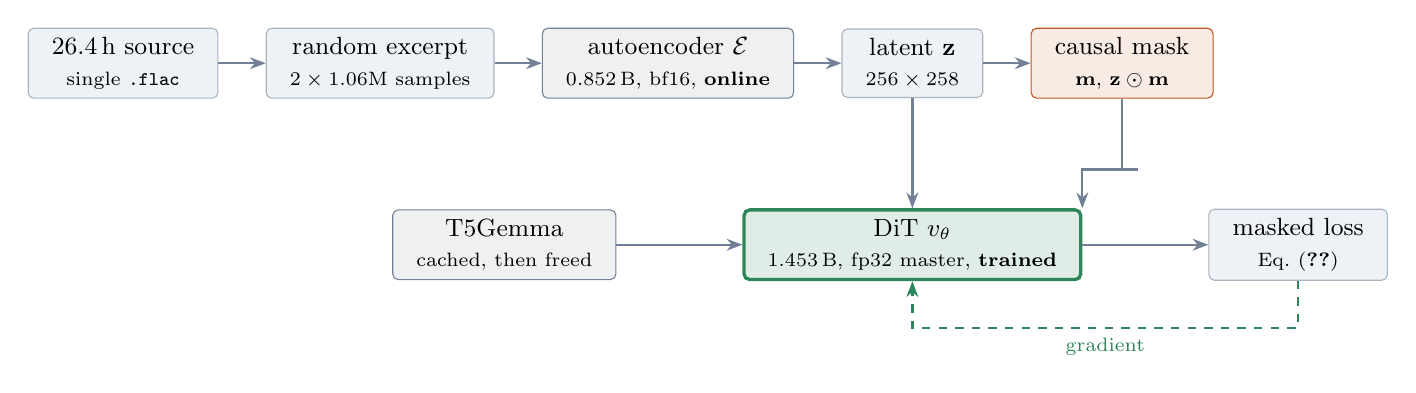
\begin{tikzpicture}[
  node distance=6mm,
  box/.style={draw,rounded corners=2pt,minimum height=8mm,align=center,font=\small,inner xsep=3mm},
  frozen/.style={box,fill=frz!12,draw=frz},
  trained/.style={box,fill=trn!15,draw=trn,very thick},
  data/.style={box,fill=bg,draw=frz!60},
  ar/.style={-{Stealth[length=2mm]},frz,thick},
]
\node[data] (src) {26.4\,h source\\\scriptsize single \texttt{.flac}};
\node[data,right=of src] (exc) {random excerpt\\\scriptsize $2\times1.06$M samples};
\node[frozen,right=of exc] (ae) {autoencoder $\mathcal{E}$\\\scriptsize 0.852\,B, bf16, \textbf{online}};
\node[data,right=of ae] (lat) {latent $\bz$\\\scriptsize $256\times258$};
\node[box,fill=gen!12,draw=gen,right=of lat] (mask) {causal mask\\\scriptsize $\bm$, $\bz\odot\bm$};

\node[trained,below=14mm of lat] (dit) {DiT $v_\theta$\\\scriptsize 1.453\,B, fp32 master, \textbf{trained}};
\node[frozen,left=16mm of dit] (txt) {T5Gemma\\\scriptsize cached, then freed};
\node[data,right=16mm of dit] (loss) {masked loss\\\scriptsize Eq.~\eqref{eq:loss}};

\draw[ar] (src) -- (exc);
\draw[ar] (exc) -- (ae);
\draw[ar] (ae) -- (lat);
\draw[ar] (lat) -- (mask);
\draw[ar] (lat.south) -- ++(0,-0.5) -| (dit.north);
\draw[ar] (mask.south) |- ++(0.2,-0.9) -| (dit.north east);
\draw[ar] (txt) -- (dit);
\draw[ar] (dit) -- (loss);
\draw[ar,trn,dashed] (loss.south) -- ++(0,-0.6) -| node[pos=0.25,below,font=\scriptsize,trn] {gradient} (dit.south);
\end{tikzpicture}
\caption{\textbf{System overview.} Grey blocks are frozen, green is trained. Nothing is
precomputed: each step reads fresh audio off disk and encodes it in the same step it is
used. The text encoder is evaluated once and then released, since its output is constant
for a run.}
\label{fig:system}
\end{figure*}

% ==========================================================================
\section{Data path}
\label{sec:data}

Conventional latent-diffusion training precomputes latents into a cache. Stability's own
configuration does this (\texttt{pre\_encoded: true}). We deliberately do not, and the
data path is correspondingly trivial: on each item we open the source file, seek to a
uniformly random frame offset, and read exactly the excerpt we need.

This has three consequences worth stating. First, there is no preprocessing stage, no
manifest, and no cache to invalidate when the excerpt length or sample rate changes.
Second, memory is independent of corpus size --- a $26.4$-hour, $10.5$\,GB source file
costs nothing to hold because it is never held. Third, the excerpt distribution is
continuous rather than quantised to cache-entry boundaries, so the model sees a different
alignment of musical structure on every epoch.

The cost is negligible: a random seek-and-decode of a $24$\,s excerpt from a $10.5$\,GB
FLAC takes $31$\,ms, and two dataloader workers hide it entirely behind GPU work.

\begin{algorithm}[t]
\caption{One training step}
\label{alg:step}
\begin{algorithmic}[1]
\State $\bx \gets$ \textsc{RandomExcerpts}(source, $B$, $\tau$) \Comment{31\,ms, on workers}
\State $\bz \gets \mathcal{E}(\bx)$ \Comment{online, bf16, no grad}
\State $\bm \gets$ \textsc{CausalMask}($B$, $T$; $p_{\text{full}}$)
\State $t \gets \sigma_L(1 - \mathrm{TLN}())$
\State $\bef \sim \mathcal{N}(0,I)$
\State $\bz_t \gets (1-t)\bz + t\bef$; \quad $v^\star \gets \bef - \bz$
\State $\hat v \gets v_\theta(\bz_t, t, c, \bm, \bz \odot \bm)$ \Comment{cfg dropout 0.1}
\State $\mathcal{L} \gets \|(\hat v - v^\star)\odot(1-\bm)\|^2 / \textstyle\sum(1-\bm)$
\State backward; clip to $1.0$; AdamW8bit step
\end{algorithmic}
\end{algorithm}

% ==========================================================================
% ==========================================================================
\section{The optimiser is part of the recipe}
\label{sec:opt}

The shipped configuration asks for \texttt{MuonAdamW}: Muon on the attention and
feed-forward matrices, AdamW on everything else. Substituting AdamW throughout is
not a neutral simplification.

Muon orthogonalises the momentum buffer before applying it. Writing $M$ for the
buffer of a matrix parameter $W \in \mathbb{R}^{m\times n}$ and $\mathrm{NS}_5$
for five steps of the quintic Newton--Schulz iteration,
\begin{equation}
W \leftarrow W - \eta\,\sqrt{\max(1, m/n)}\ \mathrm{NS}_5\!\big(M + \mu\,G\big),
\label{eq:muon}
\end{equation}
so the update has unit spectral norm by construction and $\eta$ \emph{is} the size
of the step, in the same units, for every matrix in the network. Under AdamW the
step size is set by the ratio of the gradient to its own running second moment,
which varies by more than an order of magnitude across a transformer's matrices.
A single AdamW learning rate is therefore simultaneously too large for some
matrices and too small for others, and the finetune degrades the model along the
first group while failing to move it along the second. This is the mechanism
behind a finetune whose loss falls while its samples get worse, and it compounds
with the checkpoint error of \S\ref{sec:checkpoint}.

Fused projections are split before orthogonalisation: a stacked $qkv$ weight is
several independent matrices and treating the stack as one is wrong. The
configuration's \texttt{fused\_layer\_patterns} field exists for exactly this.
The momentum buffer is held in bfloat16, which halves its cost to $2.9$\,GB and
is harmless because only the direction of \eqref{eq:muon} survives.

We also restore the exponential moving average the configuration specifies,
$\beta = 0.9995$ under a power-law warmup, and sample from it. It is kept in host
memory and updated every eighth step, which costs a copy and returns $2.9$\,GB of
device memory.

\section{Fitting a full finetune on one GPU}
\label{sec:memory}

Training all $1.453$\,B transformer parameters naively is out of reach: float32 weights,
float32 gradients and float32 Adam moments alone require
$1.453\text{B} \times 16\,\text{B} = 23.2$\,GB, before activations, before the
autoencoder, and before the text encoder. Three choices bring it inside $24$\,GB.

\begin{enumerate}\itemsep2pt
\item \textbf{Eight-bit Adam moments.} The optimiser state drops from $11.6$\,GB to
$2.9$\,GB. Master weights and gradients stay in float32, so the update itself is
unaffected in precision where it matters.
\item \textbf{The frozen autoencoder in bfloat16.} It never receives gradients, so half
precision costs nothing and saves $1.7$\,GB.
\item \textbf{Gradient checkpointing} throughout the transformer.
\end{enumerate}

Releasing the text encoder after its single use recovers a further $1.2$\,GB. The
resulting measured peak is $15.7$\,GiB, leaving comfortable headroom for the sampling
and decoding done during periodic demos.

\begin{figure}[t]
\centering
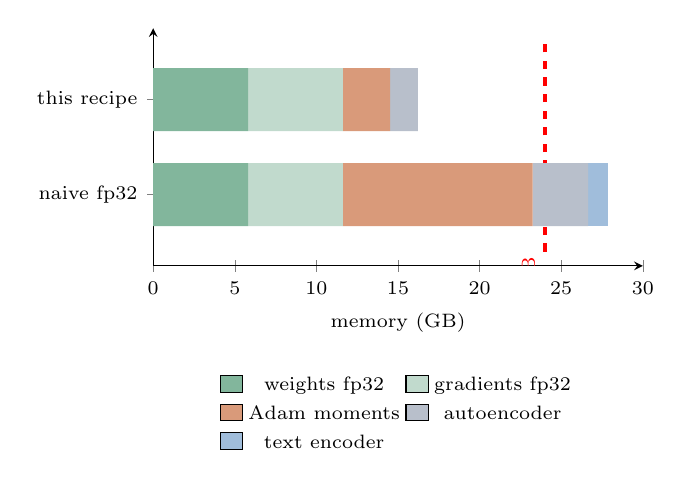
\begin{tikzpicture}
\begin{axis}[
  width=7.8cm, height=4.6cm,
  xbar stacked,
  xmin=0, xmax=30, ymin=-0.75, ymax=1.75,
  xlabel={memory (GB)},
  ytick={0,1},
  yticklabels={naive fp32, this recipe},
  tick label style={font=\scriptsize},
  label style={font=\scriptsize},
  legend style={font=\scriptsize,draw=none,at={(0.5,-0.42)},anchor=north,legend columns=2},
  axis lines=left,
  bar width=8mm,
]
\addplot[fill=trn!60,draw=none] coordinates {(5.81,0) (5.81,1)};
\addlegendentry{weights fp32}
\addplot[fill=trn!30,draw=none] coordinates {(5.81,0) (5.81,1)};
\addlegendentry{gradients fp32}
\addplot[fill=gen!60,draw=none] coordinates {(11.62,0) (2.9,1)};
\addlegendentry{Adam moments}
\addplot[fill=frz!50,draw=none] coordinates {(3.41,0) (1.70,1)};
\addlegendentry{autoencoder}
\addplot[fill=ctx!45,draw=none] coordinates {(1.20,0) (0.0,1)};
\addlegendentry{text encoder}
\draw[red,dashed,very thick] (axis cs:24,-0.6) -- (axis cs:24,1.6);
\node[red,font=\scriptsize,anchor=south east,rotate=90] at (axis cs:24,-0.55) {24\,GB};
\end{axis}
\end{tikzpicture}
\caption{\textbf{Memory budget.} Eight-bit optimiser moments, a bfloat16 frozen
autoencoder and releasing the text encoder move a $27.9$\,GB configuration to a measured
$15.7$\,GiB peak. Activations under gradient checkpointing are small and not shown
separately.}
\label{fig:mem}
\end{figure}

\subsection{Checkpoint transport}

The released checkpoint is $9.2$\,GB of float32 across $997$ tensors ($1.453$\,B
transformer, $0.852$\,B autoencoder). Since training holds float32 master weights in
memory regardless, storing bfloat16 on disk costs a single rounding at load. We therefore
convert during download, streaming tensors in file order and writing a bfloat16
safetensors file directly, so the float32 artefact is never materialised. The stored
model is $4.6$\,GB.

% ==========================================================================
\section{Cost structure}
\label{sec:cost}

\begin{table}[t]
\centering
\small
\begin{tabular}{lr}
\toprule
Stage & Time (s) \\
\midrule
Excerpt read and decode (2 workers) & 0.03 \\
Autoencoder encode (online) & 4.00 \\
DiT forward + backward & 0.45 \\
Optimiser step & $<0.01$ \\
\midrule
\textbf{Total per step} & \textbf{4.70} \\
\bottomrule
\end{tabular}
\caption{Measured per-step cost, RTX 3090, batch 4, 24\,s excerpts.}
\label{tab:cost}
\end{table}

The autoencoder dominates, costing roughly nine times the transformer step it feeds.
This is the honest price of online encoding, and it follows directly from the
architecture: a $0.852$\,B encoder that must process $8085$ patch tokens to emit $258$
latent frames does substantially more work than a $1.453$\,B transformer operating on
those $258$ frames.

\begin{figure}[t]
\centering
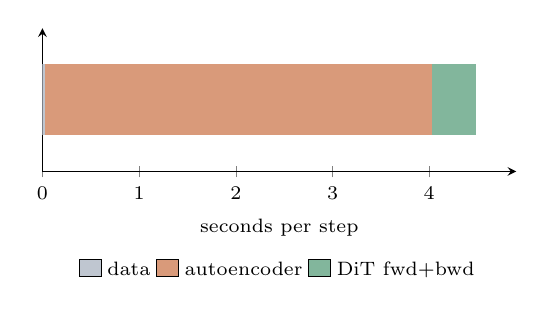
\begin{tikzpicture}
\begin{axis}[
  width=7.6cm, height=3.4cm,
  xbar stacked,
  xmin=0, xmax=4.9, ymin=-0.75, ymax=0.75,
  xlabel={seconds per step},
  ytick=\empty,
  tick label style={font=\scriptsize},
  label style={font=\scriptsize},
  legend style={font=\scriptsize,draw=none,at={(0.5,-0.55)},anchor=north,legend columns=3},
  axis lines=left,
  bar width=9mm,
]
\addplot[fill=frz!45,draw=none] coordinates {(0.03,0)};
\addlegendentry{data}
\addplot[fill=gen!60,draw=none] coordinates {(4.00,0)};
\addlegendentry{autoencoder}
\addplot[fill=trn!60,draw=none] coordinates {(0.45,0)};
\addlegendentry{DiT fwd+bwd}
\end{axis}
\end{tikzpicture}
\caption{\textbf{Where the step goes.} Online encoding is $85\%$ of wall clock. The
trade is deliberate: it buys a pipeline with no preprocessing stage and no cache, at
roughly $6\times$ the per-step cost of training from precomputed latents.}
\label{fig:steptime}
\end{figure}

We note that this cost is a \emph{choice}, not a constraint. The training loop consumes
$\bz$ and is indifferent to its provenance; substituting a precomputed latent cache
recovers the $4$\,s and changes nothing else. We prefer the online path for
single-corpus finetunes, where setup cost dominates total cost.

% ==========================================================================
\section{Evaluation protocol}
\label{sec:eval}

\begin{figure}[t]
\centering
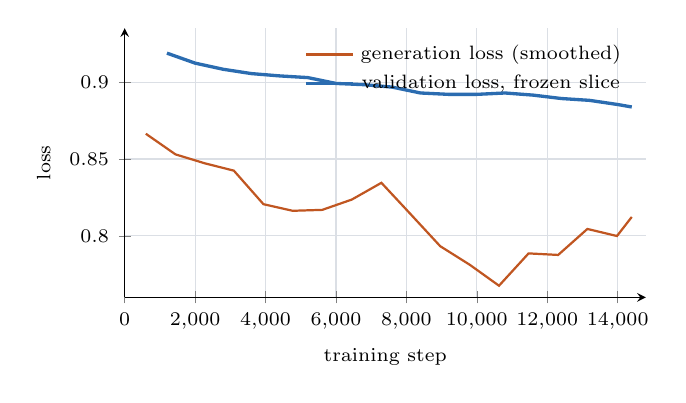
\begin{tikzpicture}
\begin{axis}[
  width=8.2cm, height=5.0cm,
  xlabel={training step}, ylabel={loss},
  xmin=0, xmax=14800, ymin=0.76, ymax=0.935,
  tick label style={font=\scriptsize}, label style={font=\scriptsize},
  legend style={font=\scriptsize,draw=none,fill=none,at={(0.98,0.98)},anchor=north east},
  axis lines=left, grid=major, grid style={frz!25},
  scaled x ticks=false, xticklabel style={/pgf/number format/fixed},
]
\addplot[gen,thick] coordinates {
(600,0.8664)(1440,0.8530)(2270,0.8472)(3100,0.8424)(3940,0.8206)(4770,0.8163)
(5610,0.8169)(6450,0.8236)(7290,0.8345)(8120,0.8141)(8960,0.7933)(9800,0.7812)
(10630,0.7676)(11470,0.7886)(12310,0.7876)(13140,0.8045)(13980,0.7999)(14400,0.8123)
};
\addlegendentry{generation loss (smoothed)}
\addplot[ctx,very thick] coordinates {
(1200,0.9188)(2000,0.9123)(2800,0.9083)(3600,0.9055)(4400,0.9040)(5200,0.9029)
(6000,0.8991)(6800,0.8983)(7600,0.8967)(8400,0.8929)(9200,0.8920)(10000,0.8920)
(10800,0.8929)(11600,0.8915)(12400,0.8893)(13200,0.8881)(14000,0.8854)(14400,0.8838)
};
\addlegendentry{validation loss, frozen slice}
\end{axis}
\end{tikzpicture}
\caption{\textbf{Both curves descend for the whole run, and neither says when to
stop.} Validation falls from $0.9275$ to $0.8838$ and is still falling at the
point where the audio evaluation (\S\ref{sec:final}) can no longer distinguish
successive checkpoints. Generation loss reaches its minimum near step $10\,600$
and then \emph{rises} while validation continues down, which is the reverse of
the usual overfitting signature and a further reason not to read either curve as
a quality measure. Neither curve would have revealed the failure of
\S\ref{sec:checkpoint}.}
\label{fig:curves}
\end{figure}

Per-step training loss is a single batch at a single randomly drawn timestep, and
rectified-flow loss depends strongly on that timestep. Over any 500-step window
of this run it spans roughly $0.75$--$0.92$, which is wider than the total
movement of the run. Reading a trend from it is guessing.

The frozen slice fixes everything that is not the model: the same four excerpts,
the same masks, the same four timesteps, the same noise. Successive values are
then directly comparable, and Figure~\ref{fig:curves} shows it falling from
$0.9275$ to $0.8891$ over 8000 steps.

\begin{table}[t]
\centering
\small
\begin{tabular}{rrr}
\toprule
Step & Validation loss & Drop per 1000 steps \\
\midrule
1     & 0.9275 & --- \\
2000  & 0.9115 & 0.0080 \\
4000  & 0.9095 & 0.0010 \\
6000  & 0.9032 & 0.0032 \\
8000  & 0.8891 & 0.0071 \\
10000 & 0.8880 & 0.0006 \\
12000 & 0.8935 & $-0.0028$ \\
14000 & 0.8804 & 0.0066 \\
\bottomrule
\end{tabular}
\caption{The frozen slice descends over the whole run, non-monotonically at this
resolution, and gives no signal at the point where the audio evaluation stops
improving.}
\label{tab:val}
\end{table}

The scalar is necessary but not sufficient. It descended smoothly through a
configuration that was measurably destroying the model (\S\ref{sec:checkpoint}),
and it was still descending at the point where doubling the training bought
nothing (\S\ref{sec:final}). We therefore evaluate on audio: a fixed reference
excerpt continued at every checkpoint, and periodically a grid of offsets drawn
from an energy gate, crossed with noise seeds, with the models under comparison
placed on identical trajectories.

That last condition is easy to get wrong. Ping-pong redraws noise inside its own
loop, so seeding the initial latent leaves two models being compared on different
paths; the measured gap between them moved by ten points of relative improvement
once the global generator was seeded as well.

% ==========================================================================
\section{Recipe summary}

Table~\ref{tab:recipe} collects every value needed to reproduce the method.
Four entries differ from the base model's own pretraining configuration: the
mask-type probabilities, reweighted toward \textsc{Causal}; the causal context
length, drawn in seconds rather than as a fraction of the window; the learning
rates, a fifth of the pretraining values because this is a finetune of a
converged model; and eight-bit moments for the AdamW group. Everything else ---
the objective, the timestep sampler, the distribution shift, the guidance dropout
rate, the optimiser pairing, the weight average --- is inherited unchanged, which
is the point.

\begin{table}[t]
\centering
\small
\begin{tabular}{ll}
\toprule
Initialisation & Stable Audio 3 Medium \textsc{Base} \\
Trained & DiT, $1.453$\,B, all parameters \\
Frozen & autoencoder $0.852$\,B, text encoder \\
Latent & $256$ ch @ $10.77$\,Hz ($/4096$) \\
Windows & $47/95/190/380$\,s, sampled per step \\
Batch & 1 $\times$ 4 accumulation \\
Objective & rectified flow, velocity target \\
Loss & generation $+$ context, Eq.~\eqref{eq:loss} \\
Mask types & $0.55$ full / $0.10$ segments / $0.35$ causal \\
Causal context & $\mathcal{U}(20, 60)$ seconds \\
Timesteps & truncated logit-normal, flipped, shifted \\
CFG dropout & $0.1$ \\
Optimiser & Muon $+$ AdamW (8-bit moments) \\
Muon & $2\!\times\!10^{-4}$, momentum $0.95$, $1.36$\,B params \\
AdamW & $10^{-5}$, $(0.9,0.95)$, wd $0.01$, $94$\,M params \\
Schedule & $200$-step warmup, $\gamma\!=\!10^6$, power $0.5$ \\
EMA & $0.9995$, power-law warmup \\
Grad clip & $1.0$ \\
Precision & fp32 master, bf16 autocast \\
Sampling & Euler $50$ steps, CFG $4$ (\textsc{Base}) \\
 & ping-pong $8$ steps, CFG $1$ (\textsc{Released}) \\
Peak memory & $20.2$\,GiB \\
Throughput & $4.4$\,s/step (RTX 3090) \\
\bottomrule
\end{tabular}
\caption{Complete hyperparameter set.}
\label{tab:recipe}
\end{table}

% ==========================================================================
\section{Results}
\label{sec:final}

We train 8000 steps on 26.4\,h of a single DJ set and merge the resulting delta
onto \textsc{Released}. Evaluation outpaints $160$\,s from a $30$\,s seed at four
offsets drawn by an energy gate, two noise seeds each, with both models placed on
\emph{identical trajectories}: ping-pong redraws noise inside its own loop, so
seeding the initial latent alone compares samplers rather than weights.

Three comparisons are worth separating, and Table~\ref{tab:final} reports all
three rather than the flattering one.

\begin{table}[t]
\centering
\small
\begin{tabular}{llrrr}
\toprule
Model & Sampler & Distance & Level & Spread \\
\midrule
\textsc{Base}, stock              & 50 step & 0.5547 & 1.10$\times$ & 0.11 \\
\textsc{Base} $+\,\Delta$         & 50 step & 0.3817 & 1.15$\times$ & 0.16 \\
\textsc{Released}, stock          & 8 step  & 0.4537 & 1.03$\times$ & 0.24 \\
\textbf{\textsc{Released} $+\,\Delta$} & \textbf{8 step} & \textbf{0.2978} & 1.11$\times$ & \textbf{0.09} \\
\midrule
the recording itself              & ---     & ---    & 1.04$\times$ & 0.33 \\
\bottomrule
\end{tabular}
\caption{Mean absolute difference between the generated region's 32-band log-mel
envelope and the true continuation's, and the ratio of generated to true RMS.
$n=8$. The merged model is $34\%$ closer than the released weights at the same
eight-step cost, winning $7$ of $8$ paired renders.}
\label{tab:final}
\end{table}

\paragraph{Against the model it started from.} At the eight steps anyone actually
samples at, the merged model scores $0.2978$ against the released checkpoint's
$0.4537$: $34\%$ closer to the true continuation, winning seven of the eight
paired renders in Figure~\ref{fig:paired}. This is the comparison that matters
for deployment, because both sides are the same architecture at the same cost.

\paragraph{Against its own many-step self.} The merged eight-step model also
beats the fifty-step model it was trained as, $0.2978$ against $0.3817$. Weights
that have been adversarially post-trained and sampled in eight steps are a better
generator than base weights sampled in fifty; the transplant makes that available
to a finetune trained under the only objective the base weights admit. The
speed-up is therefore free of a quality cost, not traded against one.

\paragraph{Reliability, not just central tendency.} The spread column is the
result we did not anticipate. The released weights produced one render at
$0.47\times$ level, a partial collapse; the merged model's worst case is
$0.96\times$, with a third of the variance ($0.09$ against $0.24$). Adding a
domain finetune to a post-trained model made it both closer on average and
markedly less prone to failing outright.

\paragraph{And where it is worse.} Figure~\ref{fig:domain} gives the other half.
On six produced songs by the same artist, held out entirely, the ordering
reverses by almost exactly the same margin: $0.4594$ against the released model's
$0.3431$. Eight thousand steps on one continuous recording buys a model that
holds that recording's groove and imposes it on everything else. That is what
specialisation is, and a result reported without this figure would be misleading.

\begin{figure}[t]
\centering
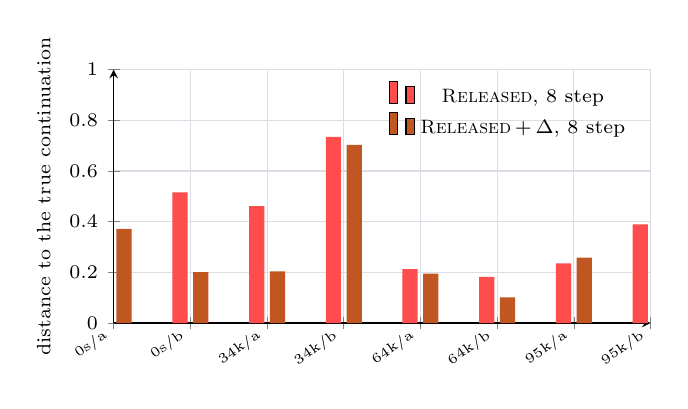
\begin{tikzpicture}
\begin{axis}[
  width=8.4cm, height=4.8cm,
  ybar, bar width=5.5pt,
  xlabel={}, ylabel={distance to the true continuation},
  symbolic x coords={{0s/a},{0s/b},{34k/a},{34k/b},{64k/a},{64k/b},{95k/a},{95k/b}},
  xtick=data, x tick label style={font=\tiny,rotate=35,anchor=east},
  ymin=0, ymax=1.0,
  tick label style={font=\scriptsize}, label style={font=\scriptsize},
  legend style={font=\scriptsize,draw=none,fill=none,at={(0.98,0.98)},anchor=north east},
  axis lines=left, grid=major, grid style={frz!25},
]
\addplot[fill=red!70,draw=none] coordinates {
({0s/a},0.8986)({0s/b},0.5152)({34k/a},0.4610)({34k/b},0.7349)
({64k/a},0.2124)({64k/b},0.1820)({95k/a},0.2358)({95k/b},0.3892)};
\addlegendentry{\textsc{Released}, 8 step}
\addplot[fill=gen,draw=none] coordinates {
({0s/a},0.3718)({0s/b},0.2014)({34k/a},0.2043)({34k/b},0.7027)
({64k/a},0.1949)({64k/b},0.1011)({95k/a},0.2580)({95k/b},0.3478)};
\addlegendentry{\textsc{Released}\,$+\,\Delta$, 8 step}
\end{axis}
\end{tikzpicture}
\caption{\textbf{Eight paired renders, identical trajectories, same eight-step
sampler.} Four offsets drawn by energy gate from the 26.4\,h source, two noise
seeds each. The finetuned model is closer to the true continuation on seven of
the eight, and its single loss is by $0.02$. The pairing matters: ping-pong
redraws noise inside its own loop, so both models must be given the same global
seed or the comparison measures the sampler rather than the weights.}
\label{fig:paired}
\end{figure}

\begin{figure}[t]
\centering
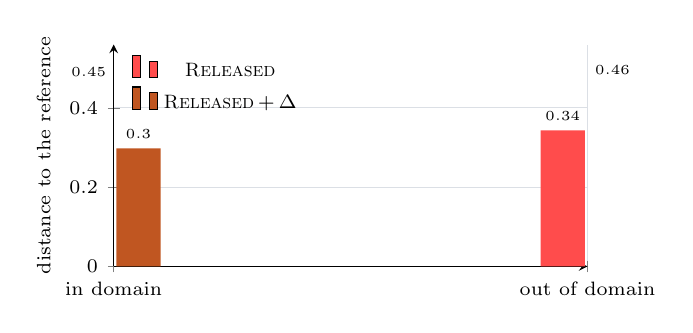
\begin{tikzpicture}
\begin{axis}[
  width=7.6cm, height=4.4cm,
  ybar, bar width=16pt,
  ylabel={distance to the reference}, ymin=0, ymax=0.56,
  symbolic x coords={{in domain},{out of domain}},
  xtick=data, tick label style={font=\scriptsize}, label style={font=\scriptsize},
  legend style={font=\scriptsize,draw=none,fill=none,at={(0.02,0.98)},anchor=north west},
  axis lines=left, grid=major, grid style={frz!25},
  nodes near coords, nodes near coords style={font=\tiny},
]
\addplot[fill=red!70,draw=none] coordinates {({in domain},0.4537)({out of domain},0.3431)};
\addlegendentry{\textsc{Released}}
\addplot[fill=gen,draw=none] coordinates {({in domain},0.2978)({out of domain},0.4594)};
\addlegendentry{\textsc{Released}\,$+\,\Delta$}
\end{axis}
\end{tikzpicture}
\caption{\textbf{Specialisation, measured in both directions.} In domain is the
26.4\,h source the finetune was trained on; out of domain is six produced songs
by the same artist, held out entirely. The finetune is $34\%$ closer in domain
and $34\%$ further out of it. A finetune that only reported the left pair would
look like a general improvement; it is not, and the symmetry is the honest
description of what 8000 steps on one recording buys.}
\label{fig:domain}
\end{figure}

\paragraph{Stopping.} The run was stopped at 8000 steps because the same
evaluation at 4000 steps scored $0.3660$ --- inside the noise of, and marginally
ahead of, 8000. The first 2000 steps bought three times what the last 2000 did.
Validation loss was still falling when the run stopped, which is precisely why it
is the wrong instrument to stop on; this is the same lesson as
\S\ref{sec:checkpoint}, arrived at from the benign direction.

\section{Discussion}

The result we would most want carried forward is the diagnostic. Whenever a
sampler rebuilds its state from a one-step estimate --- ping-pong, restart
sampling, consistency-model sampling --- that estimate has to be a sample and not
a conditional mean, and the two are distinguishable in a single forward pass by
comparing the estimate's scale against its correlation with the truth. They
coincide for a mean predictor and separate for a sample predictor. No scalar in a
training log carries this: in our runs both loss curves descended smoothly
throughout, including across an interval in which the property was being
destroyed.

The second result is that the division of labour between the two published
checkpoints is not a compromise. The base transformer is the only one a
squared-error objective is valid against; the post-trained transformer is a
strictly better generator at the step count anyone actually samples at. Carrying
a finetune between them as a delta gives both, and
Table~\ref{tab:final} shows the merged eight-step model beating the fifty-step
model it was trained as. The margin that makes this work is finite and grows as
roughly the square root of training steps, so it is worth measuring rather than
assuming --- one transformer layer fetched by byte range is enough.

The third is that capability is often already latent in a pretrained checkpoint,
distributed across a conditioning interface trained for a broader task than the
one at hand. Stable Audio 3 was trained to inpaint; outpainting is the causal
corner of that distribution. Specialising to it is a change of \emph{sampling
weights}, not a change of model: no zero-initialised branch to warm up, no
train/inference conditioning mismatch, and a step zero that is exactly the
released model.

Three limitations are worth naming. The evaluation is a spectral-envelope
distance on eight paired renders from a single source; it correlates with what we
hear but it is not a listening study. A full finetune on one domain moves the
model away from its general prior, and the residual full-mask fraction slows this
without eliminating it. And the transplant margin was verified at $1.3\times$ and
measured at $2.3\times$ at the reported checkpoint; longer runs will need it
re-checked rather than extrapolated.

\section{Conclusion}

We presented a recipe for specialising a latent rectified-flow audio diffusion model to
outpainting, with no architectural modification, on a single consumer GPU. The method
reduces to reweighting a pretrained mask distribution, keeping the reference's two-term
objective and its orthogonalising optimiser, and choosing precisions that let $1.453$\,B
parameters train in $24$\,GB.

The result we would most want carried forward is the negative one and its instrument.
Squared-error training on an adversarially post-trained checkpoint is not merely
suboptimal; it systematically undoes the post-training, and it does so while every
scalar available during the run improves. The distinction between a sample predictor and
a conditional-mean predictor is not visible in a loss curve, but it is visible in one
forward pass, and it should be checked before and after any training that touches a
distilled checkpoint. Code is available at \url{https://github.com/mrcolo/loop-training}.

\end{document}
